\section{显微技术}

显微镜分为光学显微镜、电子显微镜、扫描隧道显微镜三种。它们三者之间除了都能放大微观结构之外,没有任何共同之处。

\begin{figure}[htbp]
	\centering
	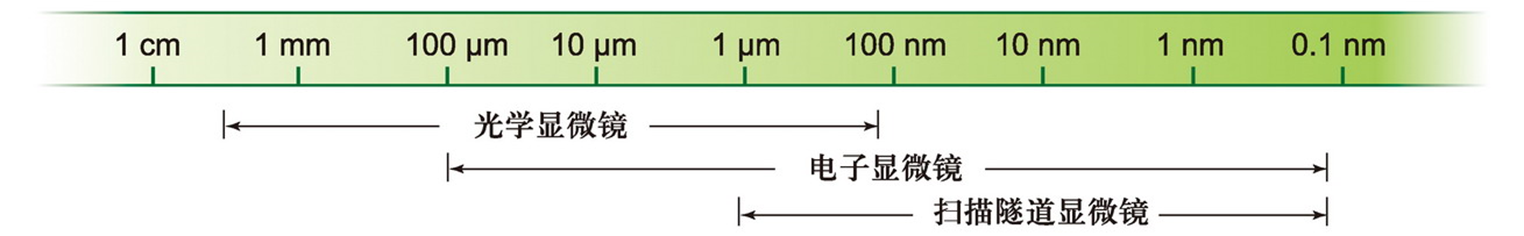
\includegraphics[width=\linewidth]{Pics/三种显微镜的分辨率范围}
	\caption{三种显微镜的分辨率范围}
	\label{fig:threeTypesOfMicroscopesResolutionRange}
\end{figure}


\subsection{光学显微镜}

\begin{figure}[htbp]
	\centering
	\begin{forest}
		forest scheme
		[光学显微镜
		[普通光学显微镜]
		[相差显微镜、微分干涉显微镜]
		[荧光显微镜]
		[激光扫描共聚焦显微镜]
		[超高分辨率显微术]]
	\end{forest}
	\caption{光学显微镜技术的分类}
	\label{fig:opticalMicroscopyTechniquesClassification}
\end{figure}

\subsubsection{分辨率和普通光镜}

分辨率是能分辨出的距离最小的两点之间的距离。分辨率\[D=\frac{0.61\lambda}{N\cdot\sin\dfrac{\alpha}{2}}\]

其中;(\autoref{fig:opticalMicroscopeResolutionInfluencingFactors})
\begin{description}
	\item[$\lambda$] 光源的波长;
	\item[$N$] 介质折射率,空气为1,香柏油为1.5;
	\item[$\alpha$] 镜口角;
	\item[NA(数值口径,镜口率)] 全称是Numerical Aperture,即$N\cdot\sin\frac{\alpha}{2}$。
\end{description}

\begin{figure}[htbp]
	\centering
	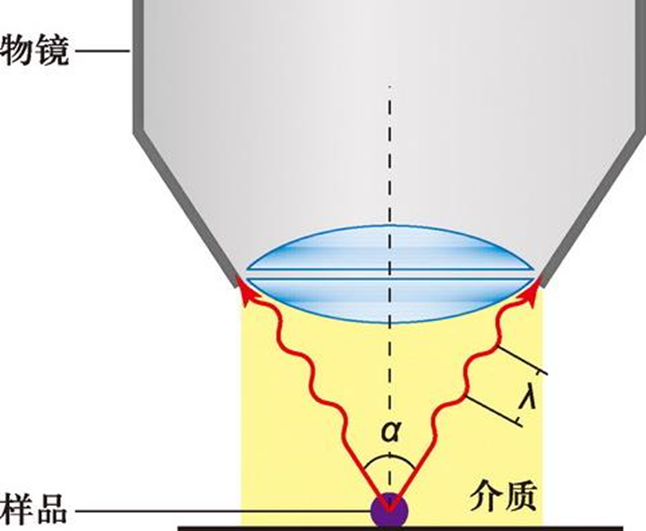
\includegraphics[width=0.4\linewidth]{Pics/光学显微镜的分辨率影响因素}
	\caption{光学显微镜的分辨率影响因素}
	\label{fig:opticalMicroscopeResolutionInfluencingFactors}
\end{figure}

光学显微镜达到最大分辨率时,以上参数分别为:
\begin{itemize}
	\item $\alpha=\SI{140}{\degree}$;
	\item 油镜下,$N=1.5$;
	\item 可见光波长最短为\SI{400}{\nm};
\end{itemize}

计算可得普通光学显微镜最大分辨率为\SI{0.2}{\um}。

\subsubsection{相差显微镜和微分干涉显微镜}

二者的比较见\autoref{tab:相差显微镜和微分干涉显微镜的比较}。

\begin{table}[htbp]
	\centering
	\begin{tabularx}{\textwidth}{|c|C|C|}
		\hline
		& \textbf{相差} & \textbf{微分干涉} \\ \hline
		原理 & 衍射与干涉 & 干涉 \\ \hline
		特殊结构 & 环状光阑与相位板 & 起偏器与合偏器 \\ \hline
		两束光来源 & 衍射 & 棱镜 \\ \hline
		相位差主要来源 & 样品不同区域密度不同 & 厚度不同 \\ \hline
		观察结果 & 明暗反差 & 浮雕状 \\ \hline
	\end{tabularx}
	\caption{相差显微镜和微分干涉显微镜的比较}
	\label{tab:相差显微镜和微分干涉显微镜的比较}
\end{table}

\subsubsection{暗视野显微镜}

聚光镜中央有挡光片,视野背景是黑的,只允许被标本反射和衍射的光线进入物镜,物体边缘是亮的。分辨率比普通显微镜高50倍。(\autoref{fig:dkfld_mcscp})

\begin{figure}[htbp]
	\centering
	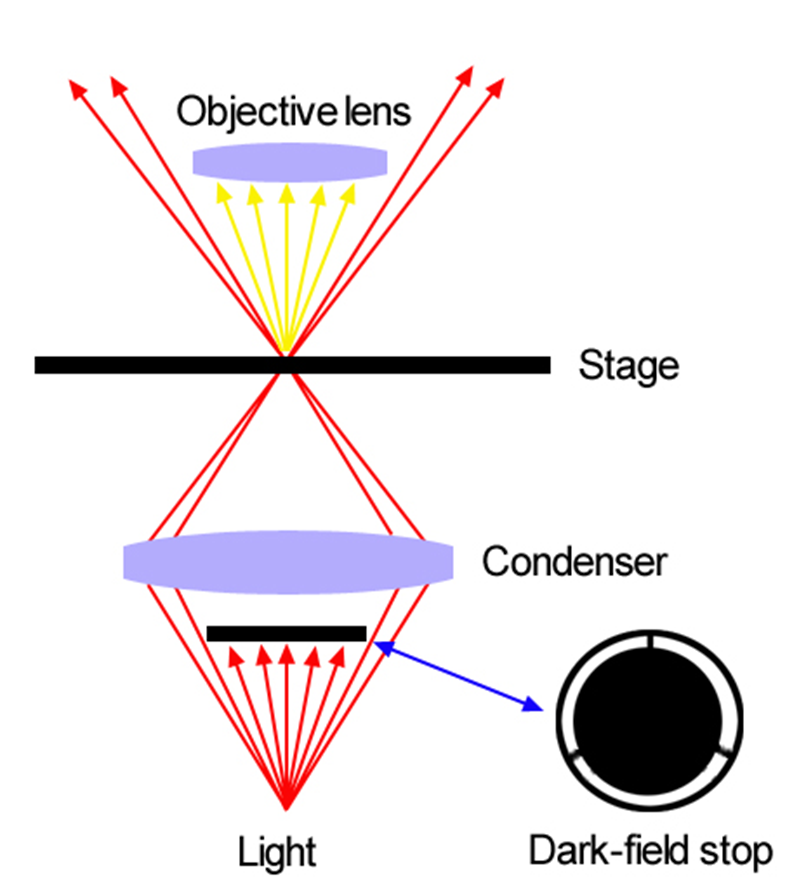
\includegraphics[width=0.4\linewidth]{Pics/暗视野显微镜}
	\caption{暗视野显微镜成像原理}
	\label{fig:dkfld_mcscp}
\end{figure}

在\autoref{fig:comparision_mcscp1}中,A图是普通光镜、B图是相差显微镜、C图是微分干涉显微镜、D图是暗视野显微镜所成的像。相差显微镜和微分干涉显微镜的成像区别是,前者边缘亮,后者有立体浮雕感。

\begin{figure}[htbp]
	\centering
	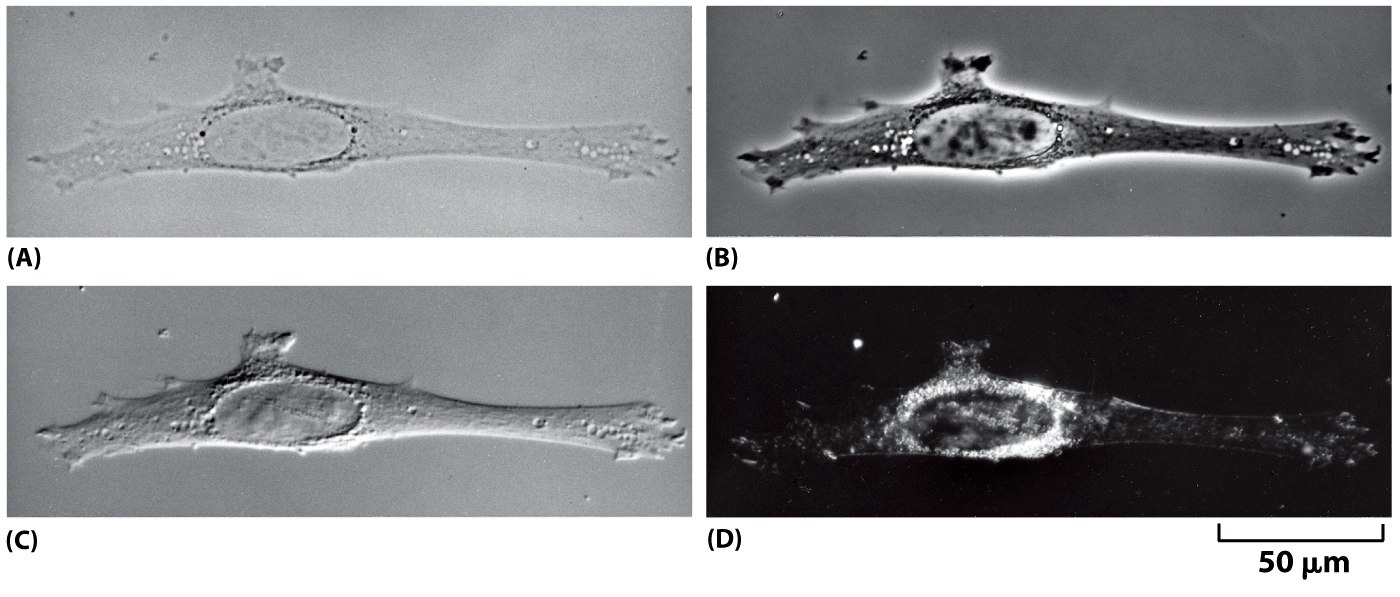
\includegraphics[width=0.8\linewidth]{Pics/显微镜成像对比}
	\caption{不同显微镜成像的对比}
	\label{fig:comparision_mcscp1}
\end{figure}

\subsubsection{荧光显微镜}

荧光显微镜的核心部件是滤光片系统和专用的物镜镜头。滤光片系统由激发滤光片和阻断滤光片组成。激发滤光片只允许特定波长的激发光通过,阻断滤光片只允许荧光染料所发出的荧光通过。(\autoref{fig:fluorescenceMicroscopeImagingPrinciple})

绿色荧光蛋白(GFP,\autoref{fig:gfp})是常用的荧光标记,只需将其与目标蛋白融合表达即可。

\begin{figure}[htbp]
	\centering
	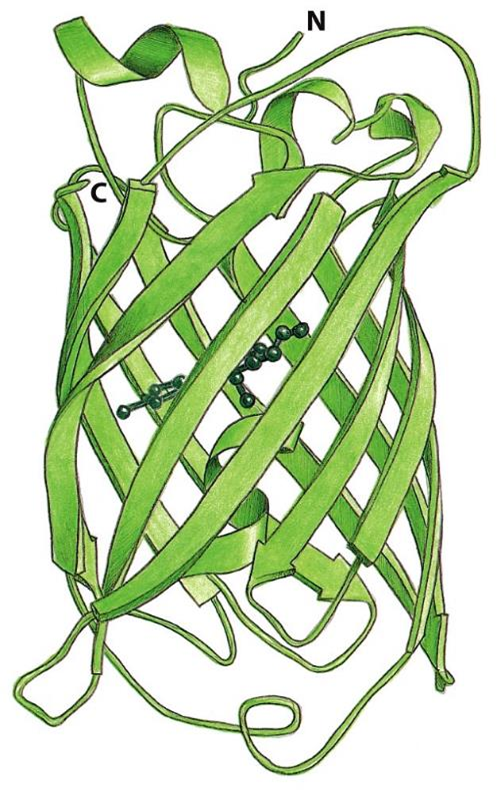
\includegraphics[width=0.3\textwidth]{Pics/GFP}
	\caption{绿色荧光蛋白的结构}
	\label{fig:gfp}
\end{figure}

\begin{gs}[:GFP与诺贝尔奖]

	\hspace{2em}马丁·查尔菲(Martin Chalfie)、钱永健、下村修(Osamu Shimomura)三人因发现GFP获得诺贝尔奖。

	\hspace{2em}道格拉斯·普瑞舍(Douglas C. Prasher)是一名美国的分子生物学家。因为他对荧光蛋白水母素 (aequorin)克隆和测序而广为科学界所知。他早年曾将他的科研经验与成果与钱永健和马丁·查尔菲 (Martin Chalfie)分享过,但是他自己却因为无法获得足够的实验经费而不得不离开学术界。最终,他完全放弃了科学工作。2008年查尔菲与钱永健因为他们对于GFP的贡献而获得诺贝尔化学奖,而他们的研究极大程度是基于普瑞舍当年的研究成果上。由于这两名诺贝尔奖得主的努力,普瑞舍终于在钱永健的资助下于2010年6月回归学术界,目前在钱永健的实验室工作。
\end{gs}

\begin{figure}[htbp]
	\centering
	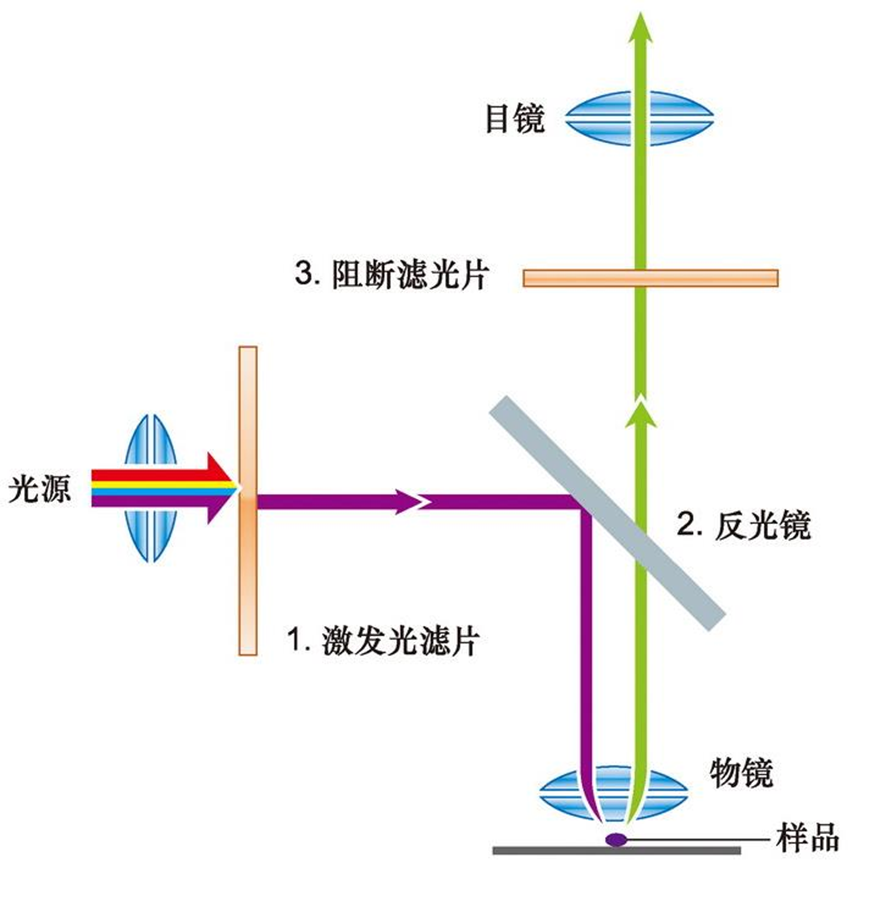
\includegraphics[width=0.4\linewidth]{Pics/荧光显微镜成像原理}
	\caption{荧光显微镜成像原理}
	\label{fig:fluorescenceMicroscopeImagingPrinciple}
\end{figure}

短波长的激发光通过激发滤光片,使样品中的荧光分子产生波长较长的荧光。荧光显微镜的暗视野提供了强反差背景,使微弱的荧光信号得以分辨。

\subsubsection{激光扫描共聚焦显微镜(LSCM)}

普通荧光显微镜下,来自不同焦平面的光线会互相干扰,导致图像模糊不清。激光扫描共聚焦显微镜相当于多安装了一套激光共焦成像系统,以激光或紫外光为光源,大大提高分辨率。共焦的意思就是,物镜和聚光镜的焦点在同一处。焦平面以外的光线就被遮挡住,因此只有来自焦平面的光线才可被观察。(\autoref{fig:LSCM},\autoref{fig:comparisonOfImagesObservedByFluorescenceMicroscopyAndLaserScanningConfocalMicroscopy})

由于观察到的画面只来自样品的一个焦平面,观察的焦平面还可以自动调整,故可以通过改变焦平面来进行“光学切片”,重构细胞的三维图像。

\begin{figure}[htbp]
	\centering
	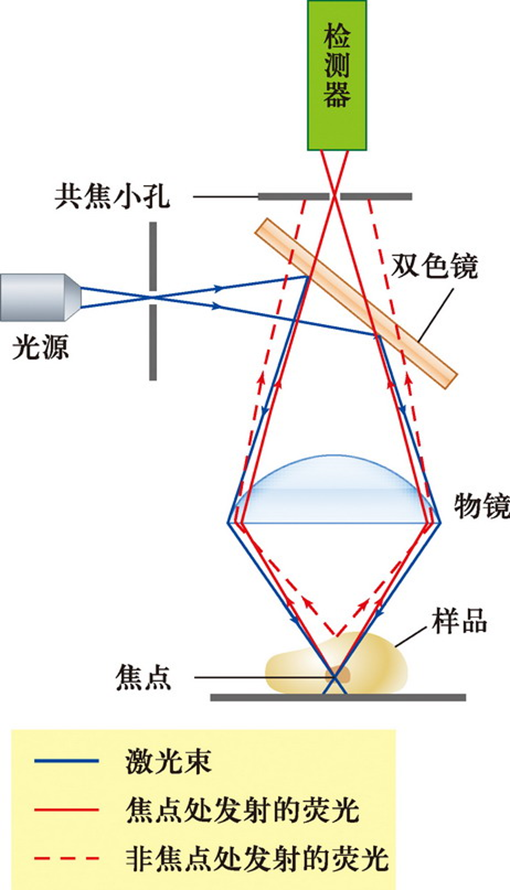
\includegraphics[width=0.3\textwidth]{Pics/激光扫描共聚焦显微镜}
	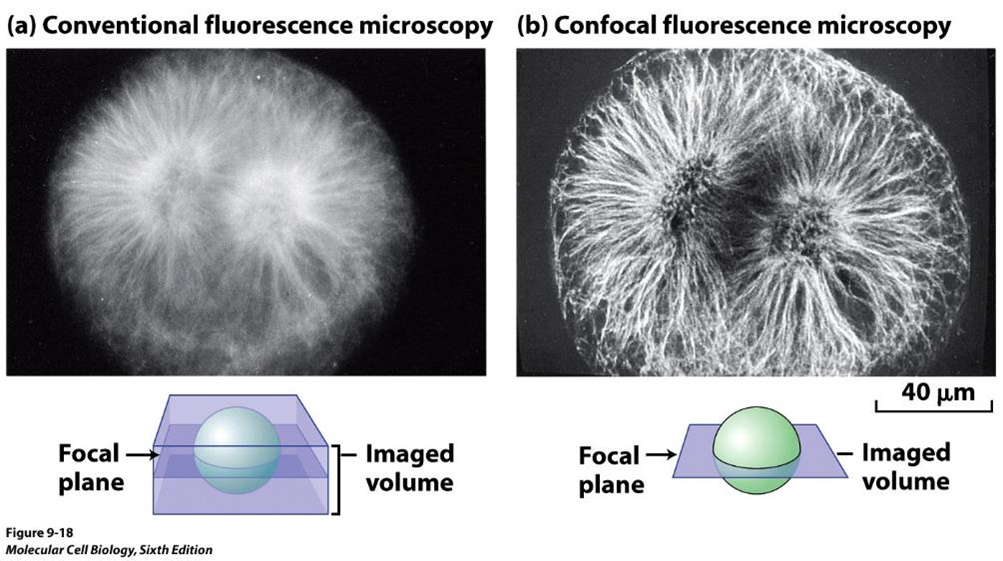
\includegraphics[width=0.5\textwidth]{Pics/激光扫描共聚焦显微镜2}
	\caption{激光扫描共聚焦显微镜成像原理}
	\label{fig:LSCM}
\end{figure}


\begin{figure}[htbp]
	\centering
	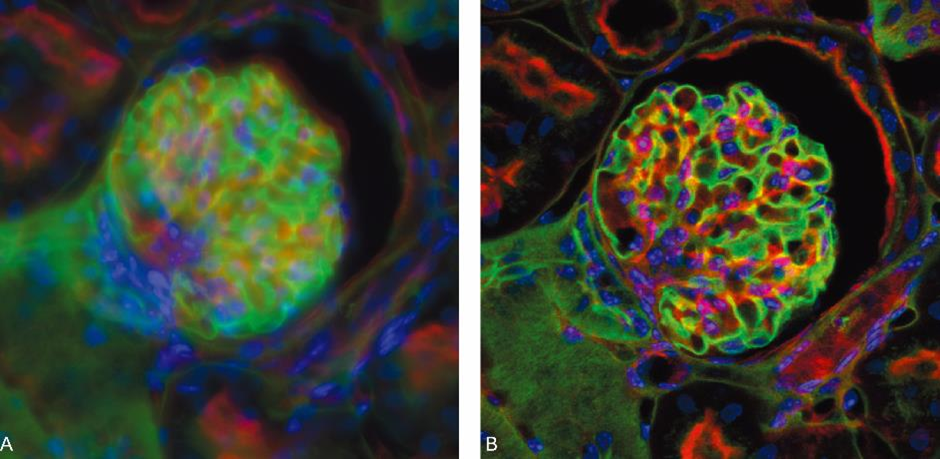
\includegraphics[width=0.7\linewidth]{Pics/荧光显微镜和激光扫描共焦显微镜所观察图像的比较}
	\caption{荧光显微镜(A)和激光扫描共焦显微镜(B)所观察图像的比较}
	\label{fig:comparisonOfImagesObservedByFluorescenceMicroscopyAndLaserScanningConfocalMicroscopy}
\end{figure}

\subsubsection{超高分辨率显微术}

在该领域,\zhongdian{我国}科学家庄小威发明了\sy{STORM技术}。它基于单分子荧光检测,在任一时刻,只有极少数荧光分子被随机激活,成像后加以精确定位。经过多次重复,由大量荧光分子的精确位点组合成了一幅STORM图像。(\autoref{fig:storm})

\begin{figure}[htbp]
	\centering
	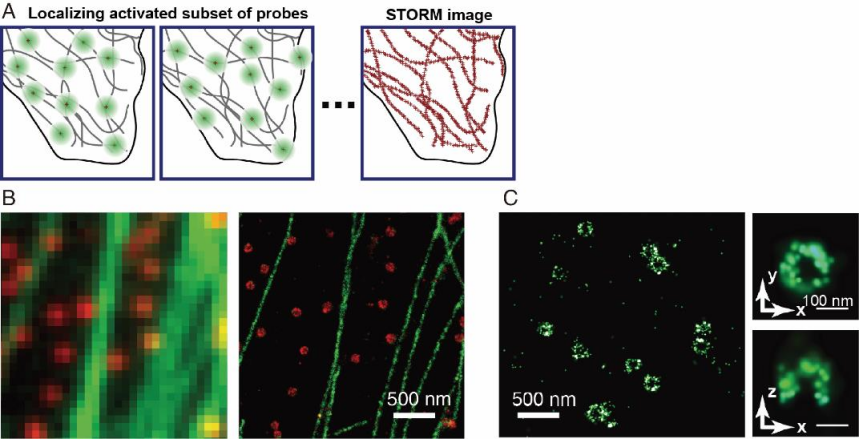
\includegraphics[width=0.7\linewidth]{STORM.png}
	\caption{STORM技术}
	\label{fig:storm}
\end{figure}

\subsection{电子显微镜}

\subsubsection{电子显微镜的基本知识}

\paragraph{与光镜的区别}

见\autoref{tab:comparisonBetweenOpticalMicroscopeAndElectronMicroscope}。

\begin{table}[htbp]
	\centering
	\begin{tabularx}{\textwidth}{|c|c|c|c|c|C|}
		\hline
		显微镜类型 & 分辨本领 & 光源 & 透镜 & 真空 & 成像原理 \\ \hline
		光学显微镜 & \SI{0.2}{\um} & 可见光 & 玻璃 & 无需 & 吸光形成明暗反差和颜色变化 \\ \hline
		电子显微镜 & \SI{0.2}{\nm} & 电子束 & 电磁 & 真空 & 电子散射和透射形成明暗反差 \\ \hline
	\end{tabularx}
	\caption{光学显微镜和电子显微镜的对比}
	\label{tab:comparisonBetweenOpticalMicroscopeAndElectronMicroscope}
\end{table}

\paragraph{电镜的分辨率}

电子显微镜的图像不可直接观察,要通过荧光屏、感光胶片或CCD来成像。

电镜的分辨率和分辨本领并不是一回事。分辨本领指的是最理想情况下的分辨率。而实际的分辨率常常受到制样技术的限制。

人眼的分辨率约为\SI{0.2}{\mm}。用人眼分辨率除以光镜和电镜的分辨率即可得到各自的放大倍数。所以,光镜的放大倍数约为1000,电镜的放大倍数约为$10^6$。

\paragraph{电子显微镜的构造}

较为原始的电子显微镜的结构如\autoref{fig:emstrctr}所示,其成像原理和现代的电镜相近。

\begin{figure}[htbp]
	\centering
	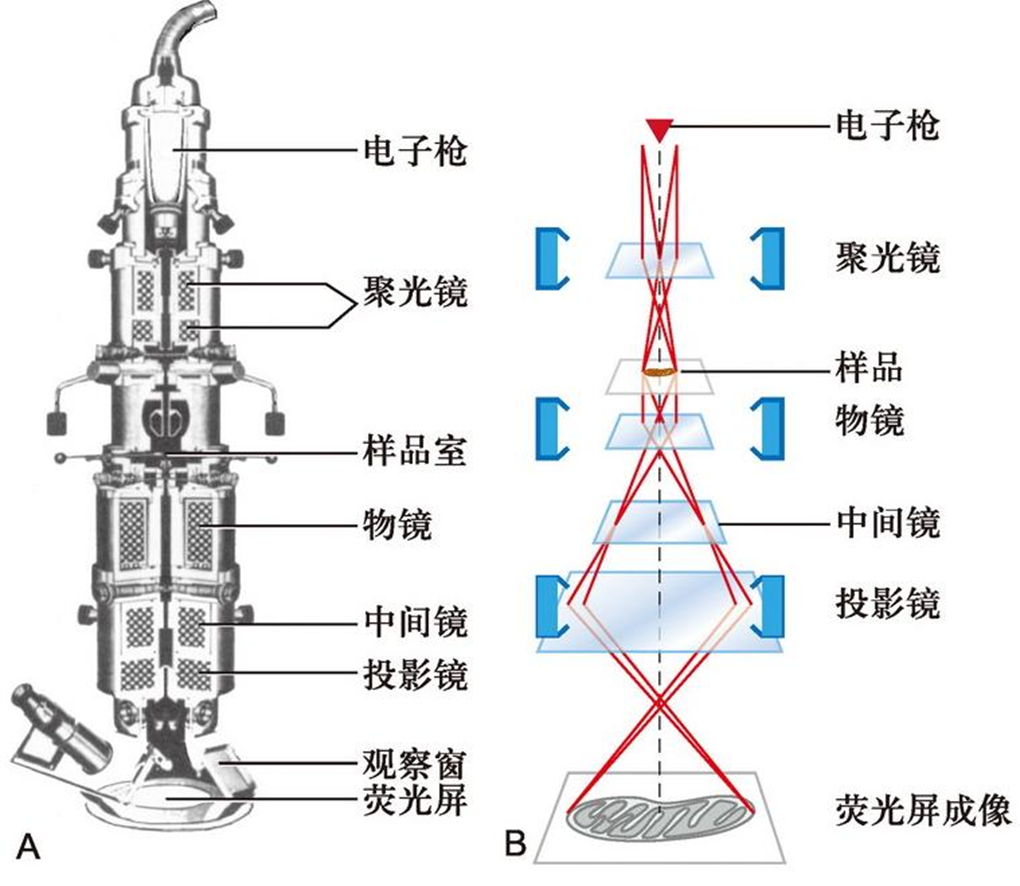
\includegraphics[width=0.5\linewidth]{Pics/EM_strctr}
	\caption{电子显微镜的结构}
	\label{fig:emstrctr}
\end{figure}

电子显微镜由以下4部分构成:
\begin{description}
	\item[电子束照明系统] 包括电子枪和聚光镜。例如,可加热钨丝发射电子,通过高电压的阳极加速电子。
	\item[成像系统] 物镜、中间镜、投影镜等精密中空圆柱体内有磁场,使电子聚焦。
	\item[真空系统] 真空泵不断抽气,保持镜筒内真空。
	\item[记录系统] 通过荧光屏、感光胶片或CCD记录。
\end{description}

\subsubsection{主要电镜制样技术}

\paragraph{超薄切片}

电子束穿透能力有限,为获得较高分辨率就要将切片变得薄,一个切片只有40\textasciitilde\SI{50}{\nm}厚。这要求样品具有一定的韧性和刚性,所以要对样品进行包埋。为了在包埋过程中尽可能保留细微结构,需要先对样品进行固定。操作流程为:固定$\longrightarrow$包埋$\longrightarrow$切片$\longrightarrow$染色。(\autoref{fig:prcs_ultr_thn_sctn})

\begin{figure}[htbp]
	\centering
	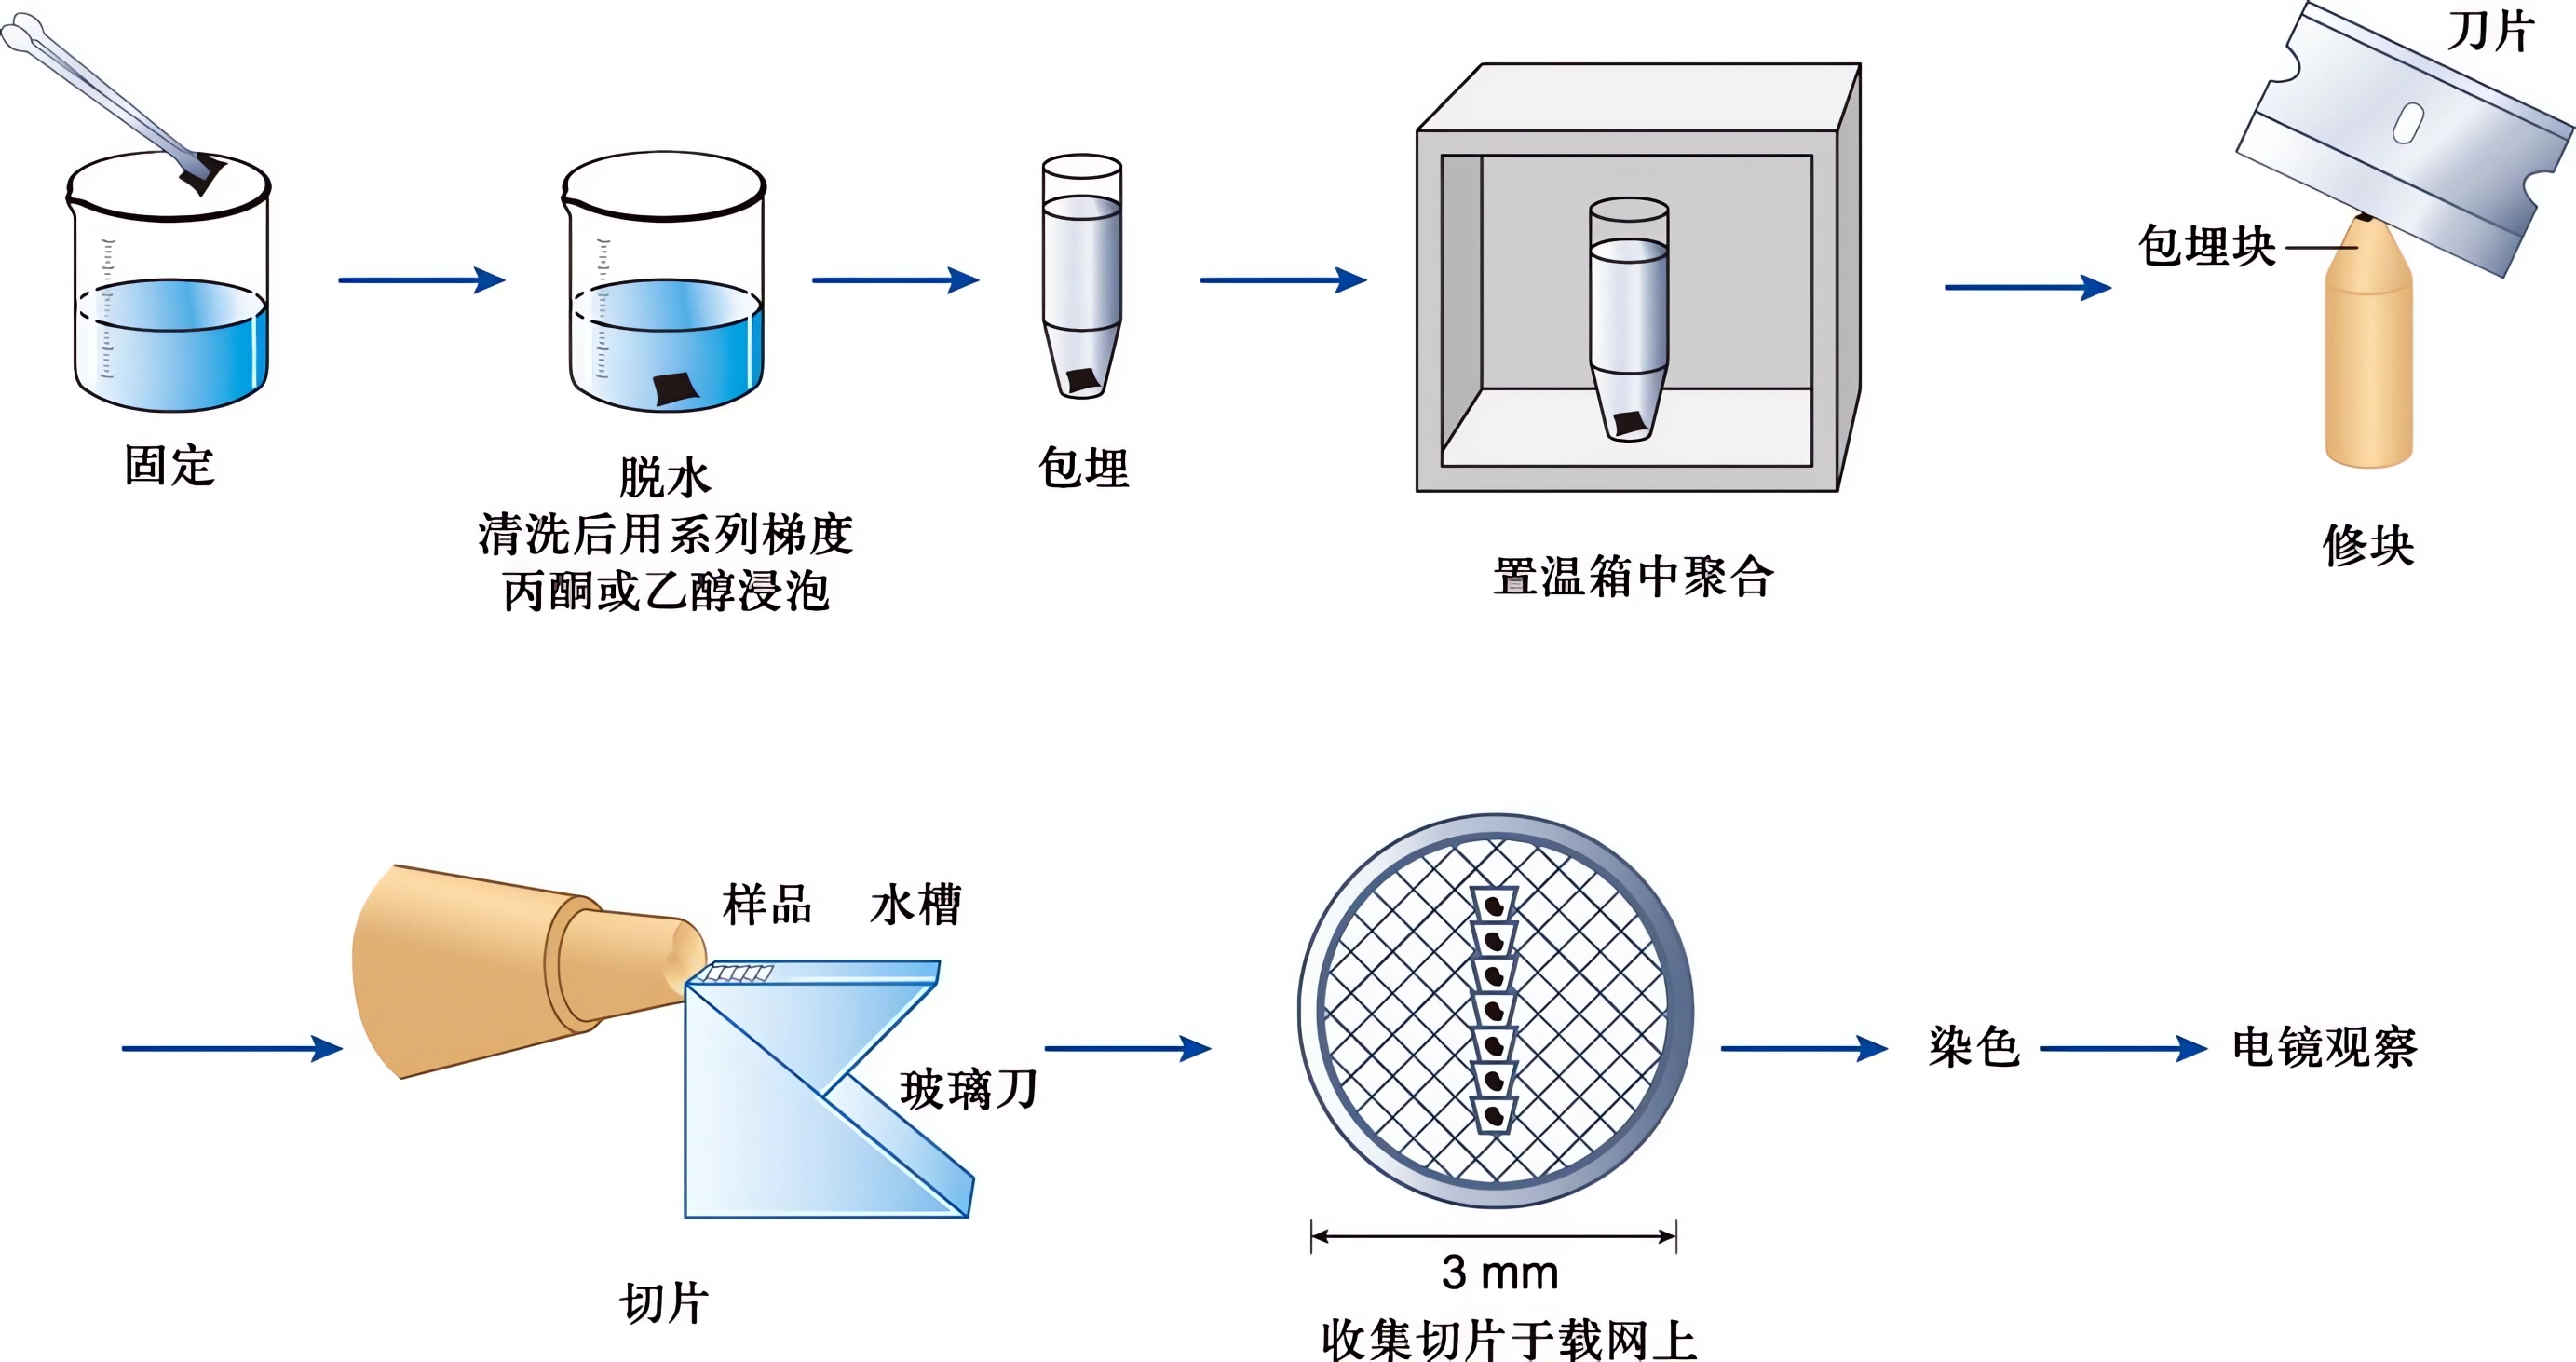
\includegraphics[width=\linewidth]{Pics/超薄切片流程}
	\caption{超薄切片流程}
	\label{fig:prcs_ultr_thn_sctn}
\end{figure}

\begin{description}
	\item[固定] 固定是保持样品真实性的最重要环节。这要求保持样品的形态和精细结构不发生改变,甚至是免疫原性不变。常用固定剂是戊二醛和锇酸(\ce{OsO4},四氧化锇)。还可额外使用冷冻等物理方法来保存细微结构。取样要快速,以防细胞结构溶解。
	\item[包埋] 包埋介质需要有良好的机械性能,以便切片。生物样品含水多,包埋剂却是疏水的,所以在包埋之前要进行脱水。常用包埋剂是各种环氧树脂。
	\item[切片] 切片常用玻璃刀或钻石刀。切片需捞在覆盖有支持膜(如Formvar膜)的载网(铜网或镍网)上。
	\item[染色] 用重金属盐染色。锇酸染脂质,柠檬酸铅染蛋白质、乙酸双氧铀染核酸。
\end{description}

应用超薄切片技术,几乎可以观察各种细胞的超微结构。

超薄切片技术还可与放射同位素自显影、细胞化学、免疫化学和原位杂交等技术结合,在超微结构水平上完成蛋白质与核酸等组分定性、定位和半定量研究。

\begin{figure}[htbp]
	\centering
	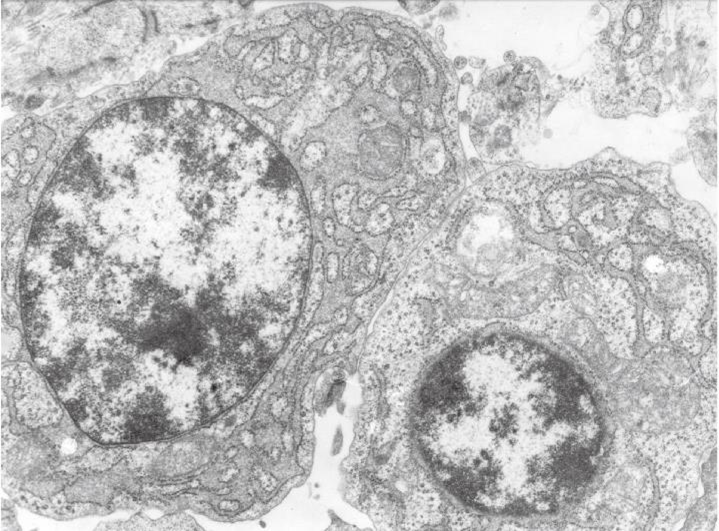
\includegraphics[width=0.5\linewidth]{Pics/超薄切片技术显示的动物细胞超微结构}
	\caption{超薄切片技术显示的动物细胞超微结构}
	\label{fig:ultrathinSectioningTechnologyShowingUltrastructureOfAnimalCells}
\end{figure}

\paragraph{负染色技术}

\begin{figure}[htbp]
	\centering
	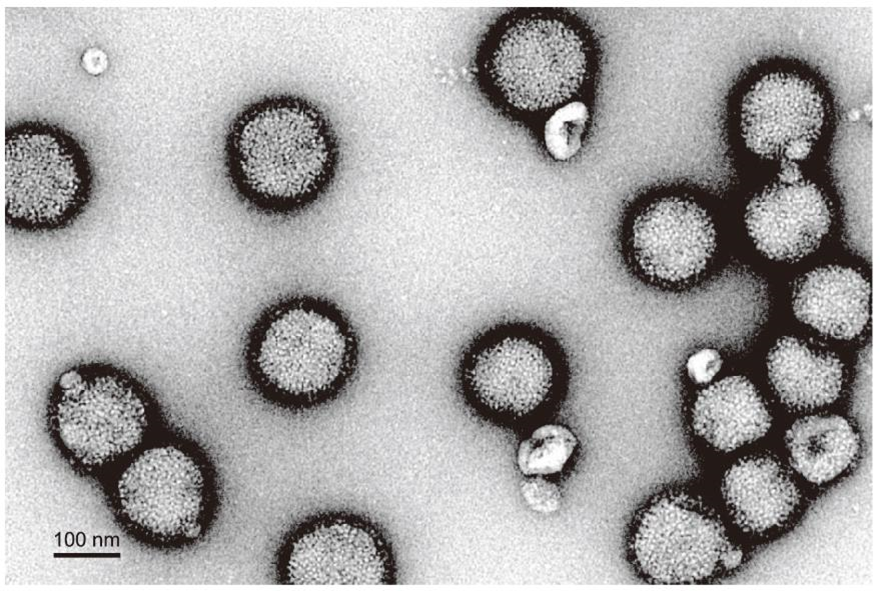
\includegraphics[width=0.5\linewidth]{Pics/流感病毒负染色电镜照片}
	\caption{流感病毒负染色电镜照片}
	\label{fig:influenzaVirusNegativeStainingElectronMicrograph}
\end{figure}


\paragraph{冷冻蚀刻技术}

\begin{figure}[htbp]
	\centering
	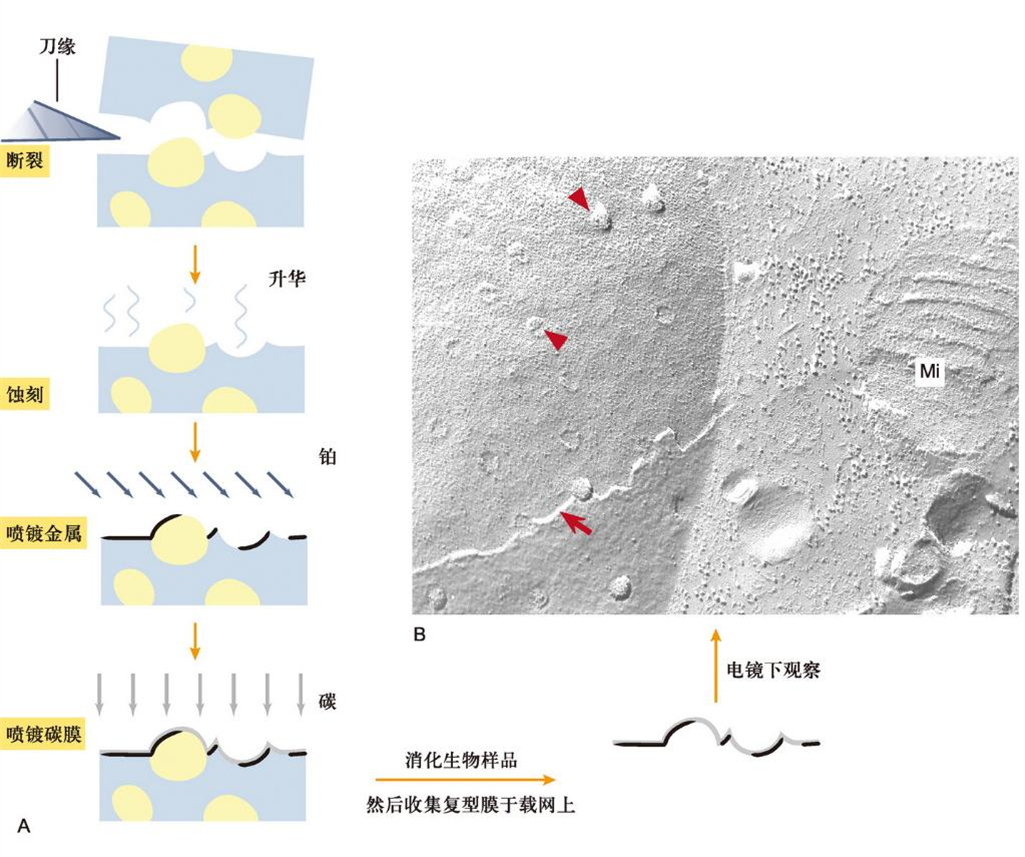
\includegraphics[width=\linewidth]{Pics/冷冻蚀刻技术示意图}
	\caption{冷冻蚀刻技术示意图}
	\label{fig:cryoFractureTechniqueSchematicDiagram}
\end{figure}

\subsubsection{不同电镜技术的对比}

如\autoref{tab:电子显微镜技术}所示。

\begin{table}[htbp]
	\centering
	\begin{tabularx}{\textwidth}{|c|c|C|C|}
		\hline
		\textbf{技术类型} & \textbf{样品制备} & \textbf{成像信息} & \textbf{观察目标} \\ \hline
		透射电镜 & 超薄切片、重金属染色 & 透射电子 & 内部层面结构 \\ \hline
		扫描电镜 & 镀金 & 二次电子 & 表面形貌 \\ \hline
		低温电镜 & 冷冻 & 透射电子 & 立体结构 \\ \hline
		电子断层成像 & 冷冻超薄切片 & 透射电子 & 层面结构 \\ \hline
		扫描背散射电子成像 & 超薄切片 & 背散射电子 & 层面结构 \\ \hline
	\end{tabularx}
	\caption{电子显微镜技术}
	\label{tab:电子显微镜技术}
\end{table}

\subsection{扫描隧道显微镜(STM)}

特点:
\begin{itemize}
	\item 具有原子尺度的高分辨率;
	\item 可以在真空、大气、液体等多种环境测量;
	\item 非破坏性测量。
\end{itemize}

原子力显微镜

\section{电泳}



\section{核酸测序}

核酸测序测的是一级结构,即碱基排列顺序。

使核酸测序发生革命性变化的因素是:
\begin{itemize}
	\item 限制性内切酶(RE)的发现,能对DNA进行特异性切割;
	\item PAGE电泳技术的发展,能分辨单个核苷酸长度差异的序列。
\end{itemize}

下面介绍四代DNA测序技术。四代DNA测序技术的总结见\autoref{tab:DNA测序技术}。

\begin{table}[htbp]
	\centering
	\begin{tabularx}{\textwidth}{|c|C|c|c|c|c|c|}
		\hline
		代数 & 名称 & 准确性 & 读长 & 通量 & 扩增 & 合成 \\ \hline
		\multirow{2}{*}{第一代} & 双脱氧法(Sanger法) & \multirow{2}{*}{{\color{red}很高}} & \multirow{2}{*}{中} & \multirow{2}{*}{极低} & \multirow{5}{*}{是} & 是 \\ \cline{2-2} \cline{7-7}
		& 化学断裂法 &  &  &  &  & {\color{red}否} \\ \cline{1-5} \cline{7-7}
		\multirow{3}{*}{第二代} & 454焦磷酸 & \multirow{3}{*}{较高} & \multirow{3}{*}{短} & \multirow{3}{*}{极高} &  & \multirow{6}{*}{是} \\ \cline{2-2}
		& Illumina/Solexa &  &  &  &  &  \\ \cline{2-2}
		& SOLiD/Applied Biosystem &  &  &  &  &  \\ \cline{1-6}
		\multirow{2}{*}{第三代} & HeliScope & \multirow{4}{*}{高} & \multirow{4}{*}{长} & \multirow{2}{*}{中等} & \multirow{4}{*}{否} &  \\ \cline{2-2}
		& 单分子实时测序(PacBio SMRT) &  &  &  &  &  \\ \cline{1-2} \cline{5-5}
		\multirow{2}{*}{第四代} & 离子流 &  &  & \multirow{2}{*}{很高} &  &  \\ \cline{2-2} \cline{7-7}
		& 纳米孔(Oxford Nanopore) &  &  &  &  & {\color{red}否} \\ \hline
	\end{tabularx}
	\caption{DNA测序技术,“扩增”指需要大量样本,“合成”指边合成边测序}
	\label{tab:DNA测序技术}
\end{table}

\subsection{第一代测序}

\subsubsection{双脱氧法}

双脱氧法也称末端终止法、Sanger法。它是最常用的第一代测序方法。具体原理见\autoref{fig:sanger_dna}。

\begin{figure}[p]
	\centering
	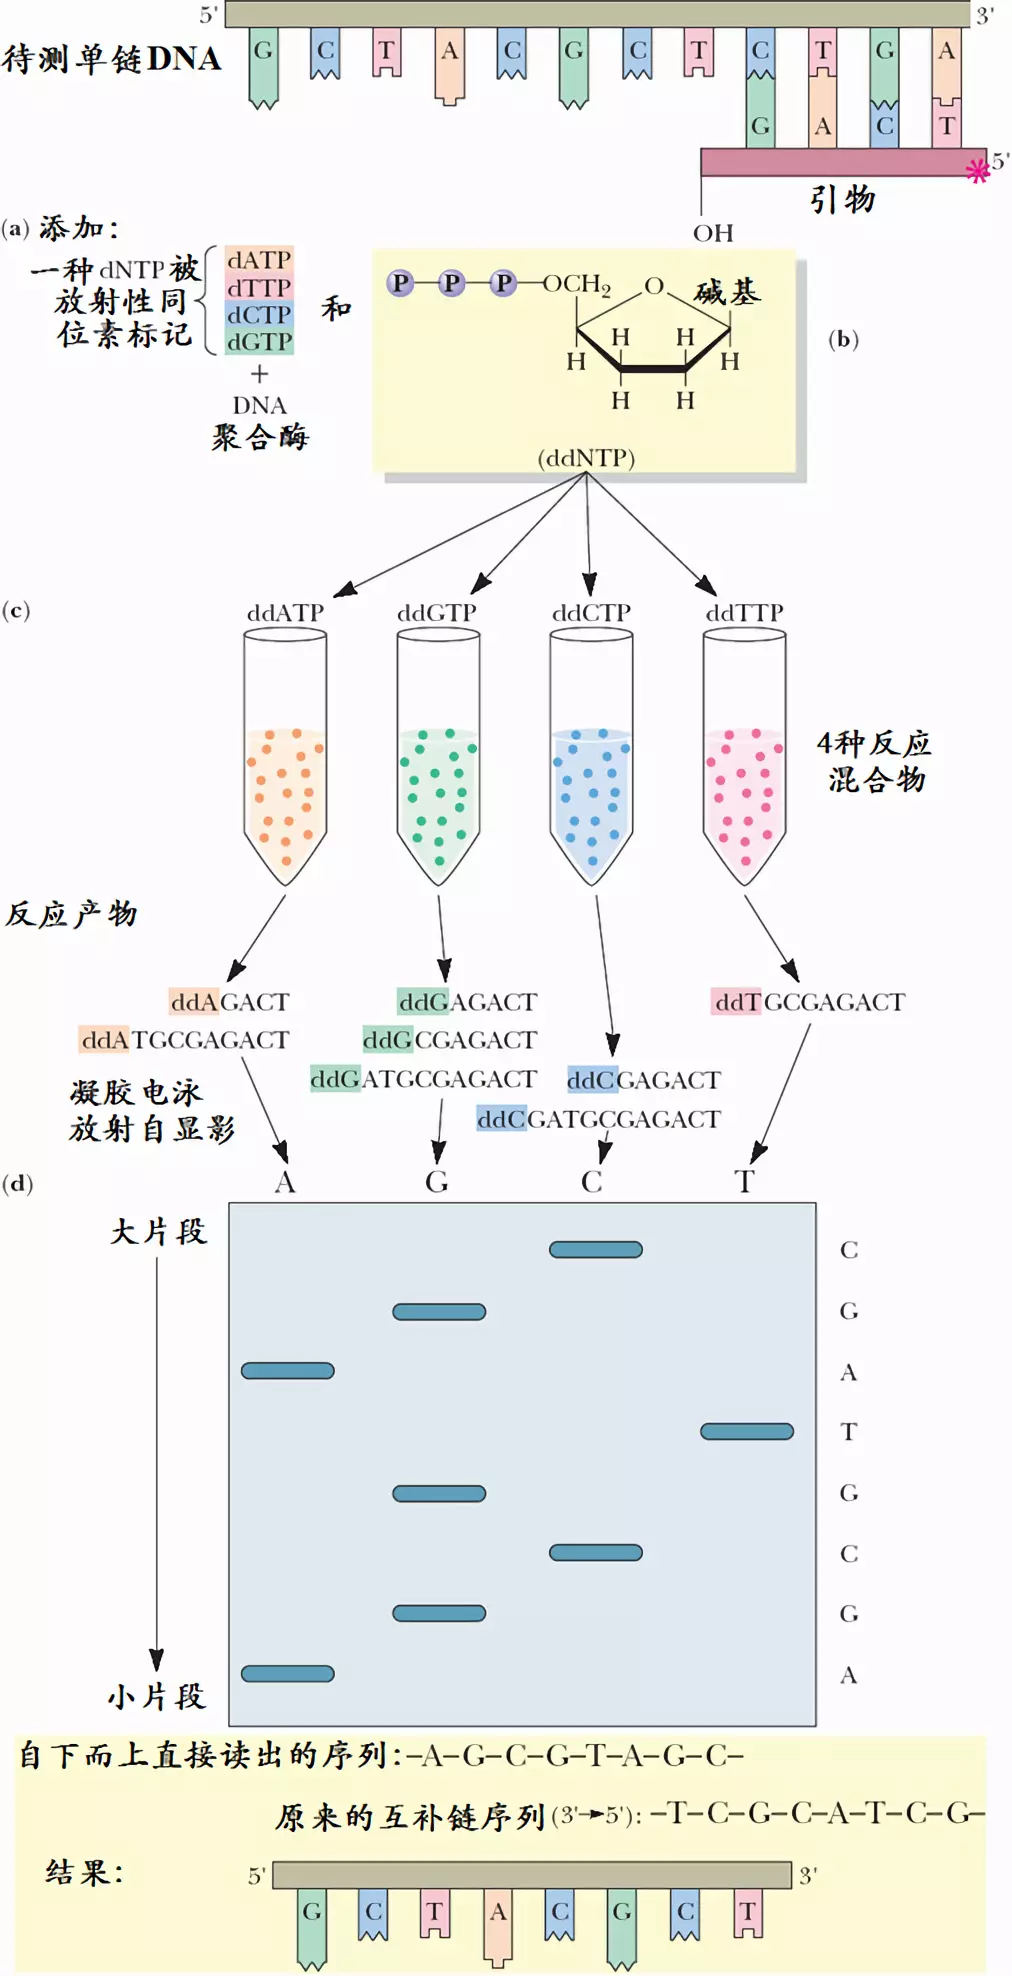
\includegraphics[width=0.7\linewidth]{Pics/Sanger法DNA测序}
	\caption{双脱氧法测序原理}
	\label{fig:sanger_dna}
\end{figure}

\subsubsection{碱基特异性化学断裂法}

又称化学断裂法、Maxam-Gilbert法。

化学断裂法需要进行四组平行的反应:

\begin{description}
	\item[G特异性剪切] 在碱性条件下,先用硫酸二甲酯(DMS)处理,然后再使用哌啶处理;
	\item[嘌呤(A+G)碱基特异性剪切] DNA先进行酸处理,然后再加DMS;
	\item[嘧啶(C+T)碱基特异性剪切] 先用肼处理,然后用哌啶处理;
	\item[C特异性剪切] 在高盐下,先用肼处理,然后用哌啶处理;
\end{description}

进行聚丙烯酰胺凝胶电泳和放射自显影。比较G、A+G、C+T和C各个泳道,自下而上从自显影片上就可读出DNA序列。

\begin{figure}[htbp]
	\centering
	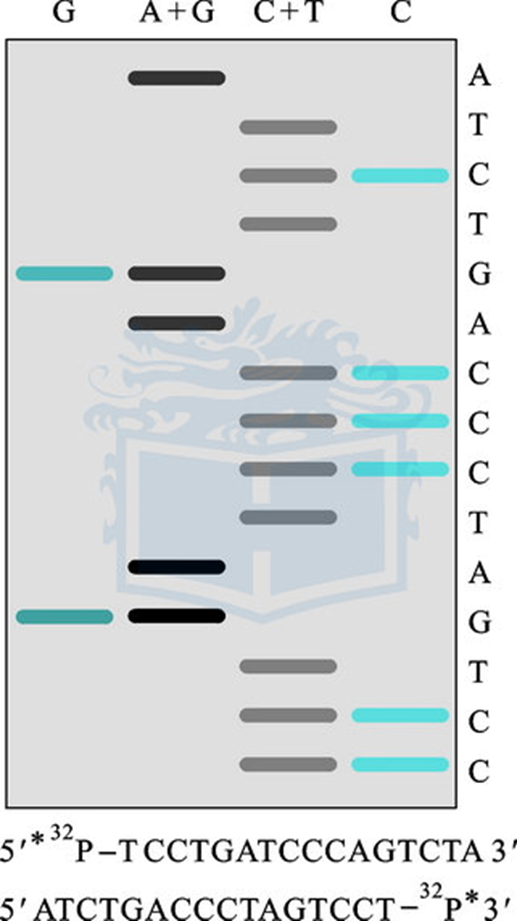
\includegraphics[width=0.3\linewidth]{Pics/化学断裂法测序}
	\caption{化学断裂法测序}
	\label{fig:MG_sequencing}
\end{figure}


\section{核酸分离、纯化、定量}

\subsection{酚-氯仿-异戊醇抽提}

细胞裂解后分离上清液,加入苯酚、氯仿、异戊醇(体积比$25:24:1$)。
\begin{itemize}
	\item 苯酚可竞争氢键,使蛋白质变性;
	\item 氯仿可以溶解苯酚等脂溶性物质,去除杂质;
	\item 异戊醇降低表面张力,消泡。
\end{itemize}

用乙醇和\ce{NaCl}沉淀DNA。
\begin{itemize}
	\item 加入\ce{Na+},可以中和DNA携带的负电荷。
\end{itemize}

75\%乙醇洗涤。

用TE buffer溶解DNA。

\subsection{质粒提取——SDS碱裂解法}

三个溶液:
\begin{description}
	\item[溶液I] 溶菌酶、\SI{50}{\mmol\per\L}葡萄糖、\SI{25}{\mmol\per\L} Tris pH 8.0,\SI{10}{\mmol\per\L}EDTA
	\begin{itemize}
		\item 溶菌酶溶解细胞壁;
		\item 葡萄糖维持溶液渗透压,防止DNA受机械剪切力损伤;
		\item EDTA可螯合金属离子,抑制DNase、促进溶菌酶的作用。
	\end{itemize}
	\item[溶液II] \SI{0.2}{\mmol\per\L} \ce{NaOH}、1\% SDS
	\begin{itemize}
		\item \ce{NaOH}调pH为碱性,使DNA变性;
		\item SDS使蛋白质变性。
	\end{itemize}
	\item[溶液III] \SI{50}{\mmol\per\L}醋酸钠、大量冰醋酸
	\begin{itemize}
		\item 形成缓冲体系,调pH至中性。
	\end{itemize}
\end{description}

后续使用酚仿抽提提取。

\subsection{RNA提取}


\subsection{核酸纯度检测}

使用Nanodrop分光光度计检测:
\begin{description}
	\item[A260/A230] \SI{230}{\nm}处是糖类、胍盐等杂质的吸收峰。纯净的核酸样品该值约为2.5。
	\item[A260/A280] 前者是核酸的吸收峰,后者是蛋白质的吸收峰,反映核酸被蛋白质污染的程度。纯净双链DNA约为1.8,RNA大于2。这一参数是最重要的。
\end{description}

浓度换算关系:1OD相当于\SI{50}{\ug\per\ml}的dsDNA、\SI{37}{\ug\per\ml}的ssDNA、\SI{40}{\ug\per\ml}的RNA。



\subsection{核酸杂交}

\subsubsection{DNA杂交——Southern Blot}


\subsubsection{RNA杂交——Western Blot}

\subsubsection{膜上印迹杂交}

\subsubsection{基因芯片}

\section{基因工程}

\subsection{分子克隆——Gateway克隆}

\subsubsection{原理和试剂}

Gateway克隆就是噬菌体感染细菌时发生的整合和切割重组反应的体外版本。噬菌体DNA上含有attP位点,细菌DNA上含有attB位点,二者发生重组使噬菌体DNA整合进细菌DNA\footnote{att, \textbf{att}achment site; P, \textbf{p}hage; B, \textbf{b}acteria}。重组后,在细菌DNA上产生新的attL和attR位点,这两个位点可以再次发生重组,“吐出”噬菌体DNA。(\autoref{fig:Gateway克隆的原理})

\begin{figure}[htbp]
	\centering
	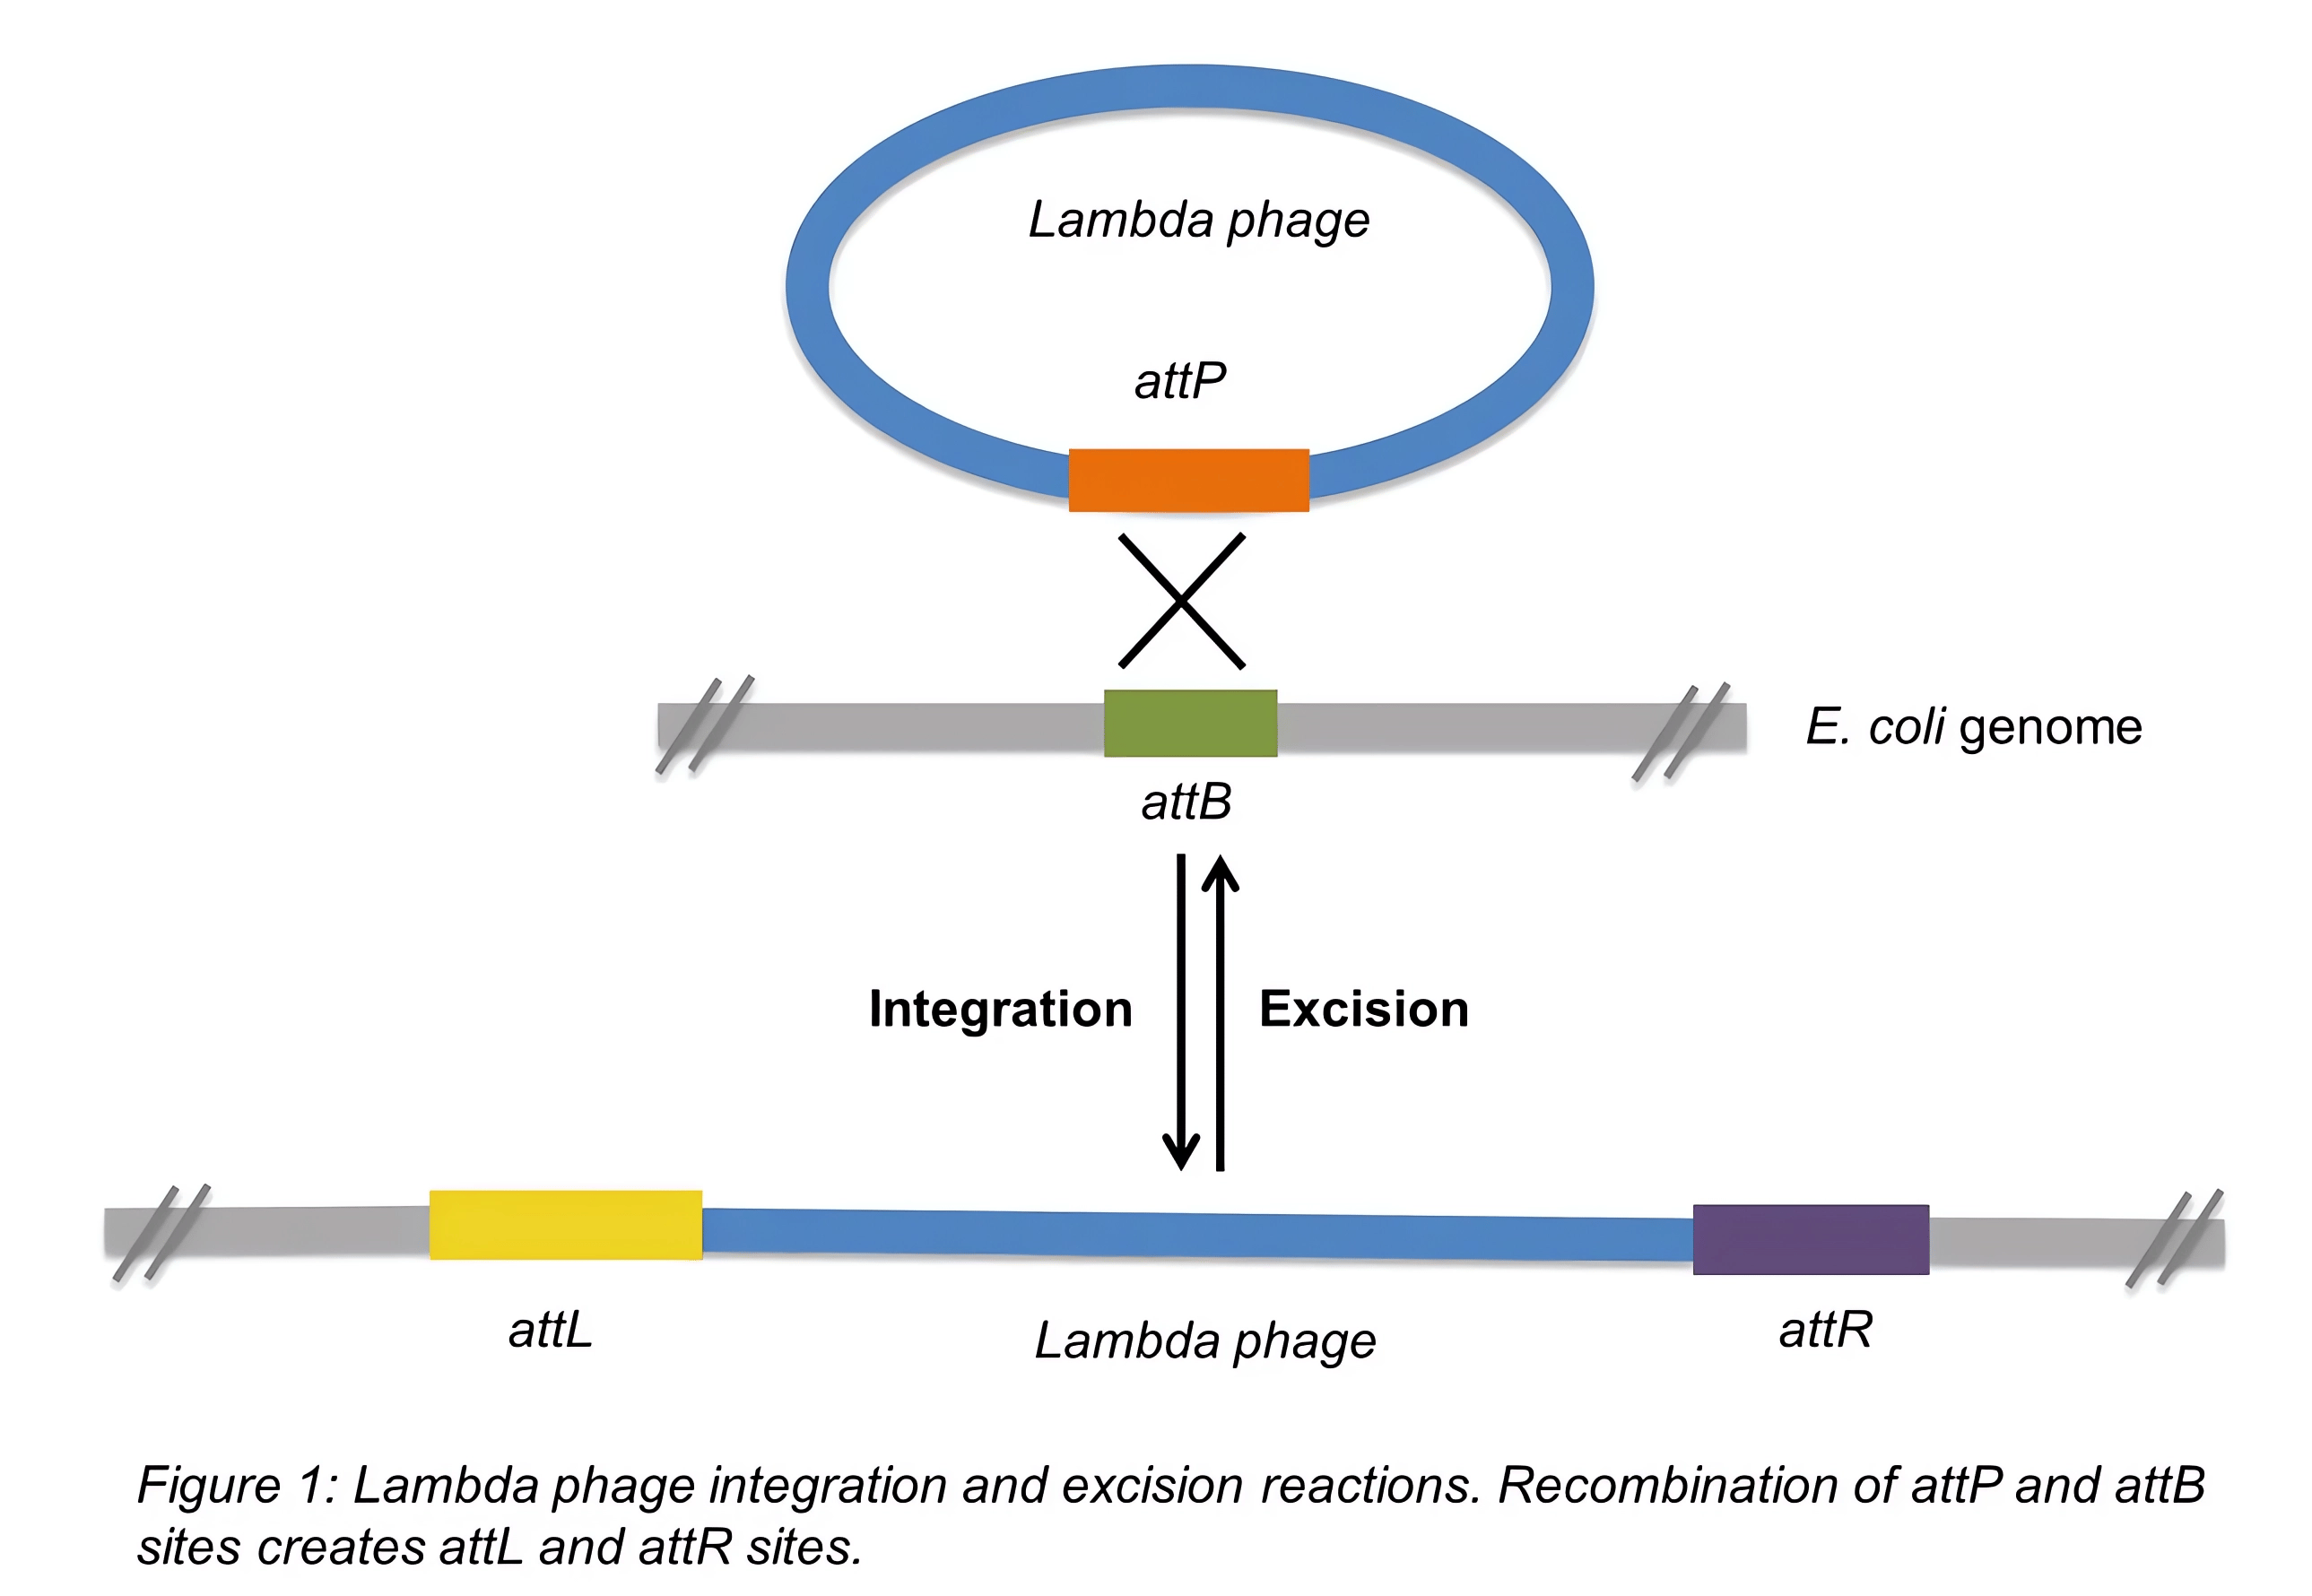
\includegraphics[width=\textwidth]{GatewayClone1.png}
	\caption{Gateway克隆的原理}
	\label{fig:Gateway克隆的原理}
\end{figure}

试剂:
\begin{itemize}
	\item 底物:
	\item 酶:商品化的BP Clonase和LR Clonase,分别催化BP反应和LR反应。
\end{itemize}

\subsubsection{反应过程}

\autoref{fig:Gateway克隆的步骤}

\begin{figure}[htbp]
	\centering
	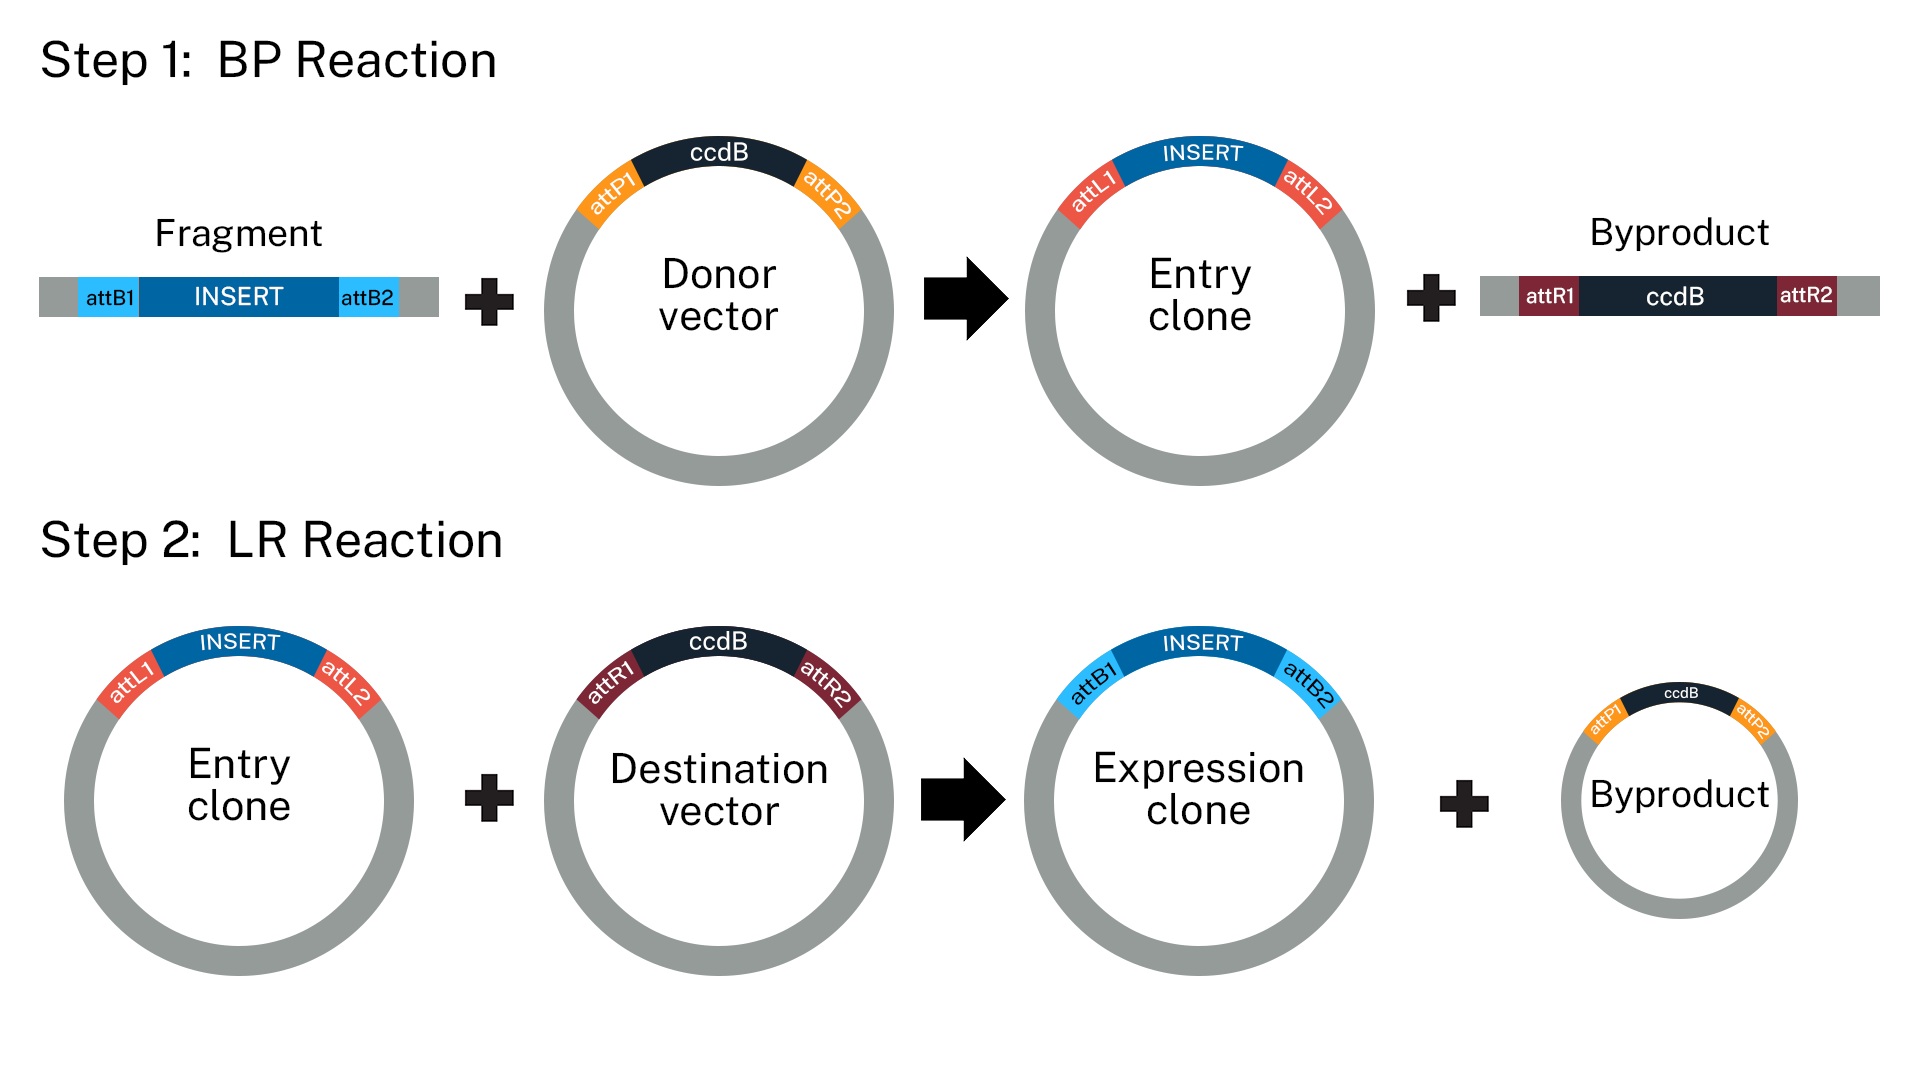
\includegraphics{GatewayClone2.png}
	\caption{Gateway克隆的步骤}
	\label{fig:Gateway克隆的步骤}
\end{figure}

\textit{ccdB}编码的蛋白质是一种毒素,破坏细菌的拓扑异构酶II,使细菌死亡。在这里作为筛选标记,成功克隆的个体,\textit{ccdB}被破坏,可以生存。

\subsection[聚合酶链式反应(PCR)]{\sy{聚合酶链式反应(PCR)}}

\paragraph{PCR的反应体系}

\begin{description}
	\item[DNA模板]
	\item[DNA引物]
	\item[DNA pol]
	\item[dNTP]
	\item[\ce{Mg^{2+}}] 这是DNA聚合酶所必须的。有时加入的是\ce{Mn^{2+}}进行易错PCR,因为DNA聚合酶的校对活性依赖于\ce{Mg^{2+}}。
\end{description}

\paragraph{PCR操作流程}

预变性




\section{蛋白质分离、纯化、定量}

\subsection{蛋白质分离纯化}

\subsection{蛋白质定量}

\subsubsection{凯氏定氮法}

蛋白质与硫酸和催化剂共热,硫酸铵与NaOH释放氨气,可测定含氮量/0.16

\subsubsection{双缩脲法}

碱性溶液中 cuso4 540nm比色 标准曲线

灵敏度较差,样品用量大。

\subsubsection{Lowry法}

福林酚显色  福林酚不是酚

660nm比色

\subsubsection{BCA法}

562nm BCA还原二价铜离子。溶液中不能含有EDTA或dtt等还原剂

\subsubsection{Bradford法}

考马斯亮蓝G-250在酸性溶液中鲜红色,与碱性氨基酸结合后蓝色。595nm

与还原剂兼容,但受去垢剂影响较大。

\subsubsection{工具——分光光度仪}

朗伯比尔光吸收定律 $A=\epsilon bc$

\subsection{蛋白质电泳}

\subsubsection{电泳准备}

竖着、

缓冲液:25mM Tris-HCl  190nMGLY
浓缩胶:偏中性,把蛋白质拉到同一条线上
分离胶:偏碱性


\section{分子互作研究}

\subsection{互作研究技术的适用范围}

\subsection{荧光偏振(FP)}

当特定波长的偏振光激发荧光分子时,分子会吸收能量并跃迁到激发态。若分子处于静止状态(如结合到大分子上),其发射的荧光会保持较高的偏振度(polarization);若分子快速旋转(如小分子自由运动),发射光的偏振度会降低。

\begin{itemize}
	\item 大分子或结合态分子:旋转速度慢,发射光偏振度高;
	\item 小分子或游离态分子:旋转速度快,偏振度低。
\end{itemize}

通过测量偏振度的变化($\upDelta$P),可判断分子是否发生了结合或构象改变

\subsection{ATAC-seq}

\section{文献阅读题中常见的缩写}

\begin{table}[htbp]
	\begin{tabularx}{\textwidth}{|c|C|C|}
		\hline
		缩写 & 全称 & 含义 \\ \hline
		OE & Over Expression & 过表达 \\ \hline
		$\updelta$ & 表示“变化”的惯用符号 & 基因敲除 \\ \hline
		KO & Knock Out & 基因敲除 \\ \hline
		:: & & 启动子::基因 \\ \hline
		XFP & \begin{tabular}[c]{@{}c@{}}Green/Yellow/Red/Cyan \\ Flourescence Protein\end{tabular} & 荧光蛋白\\ \hline
	\end{tabularx}
\end{table}